\documentclass[12pt]{article}
\usepackage[utf8]{inputenc}
\usepackage{amsmath}
\usepackage{systeme}
\usepackage{amsfonts}
\usepackage{graphicx}
\usepackage{enumitem}
\usepackage{hyperref}
\usepackage{xcolor}
\usepackage{kbordermatrix}
\usepackage{centernot}
\usepackage{xcolor}

\title{%
	\textbf{Notițe Seminar 4}}

\begin{document}
	
	\maketitle
	
	\textbf{\large{Învățare supervizată de tip clasificare (2)}}
	
	\textbf{Intro:} În seminarul trecut v-am zis că există faza de antrenare și faza de testare, însă nu v-am zis întreaga poveste, mai există și o fază de validare...
	
	\textit{Context}: cineva vă dă un set de date despre apartamente cu atribute de intrare și un atribut de ieșire și vă cere să găsiți un model ML care să se comporte cât ma bine pe date noi și să furnizați un număr care să indice acest lucru.
	
	Voi ce faceți? Vă faceți o listă cu mai mulți algoritmi (să zicem 15) (sau mai multe variante de algoritmi) pe care vreți să-i încercați (ID3, rețea neuronală, ID3 dar nu cu IG, ci cu index Gini etc) și apoi aveți cel puțin 3 opțiuni:
	\begin{enumerate}
		\item 
		\begin{enumerate}
			\item antrenați 15 modele pe setul de date pe care îl aveți coresp. celor 15 alg.
			\item calculați acuratețea pentru fiecare model la antrenare
			\item selectați modelul cu acuratețea maximă și raportați acea acuratețe
			\item Chiar dacă modelul vostru se descurcă foarte bine pe setul de date de antrenare, acest lucru nu înseamnă că el se va descurca bine pe date noi. Cel mai probabil nu o va face. Cu alte cuvinte, ați dat peste \textit{\textbf{overfitting}} (= obțineți un model care are la antrenare acuratețe mai mare decât la testare când testăm cu date noi = v-ați pliat prea mult pe datele de antrenament = ați \textit{tocit} datele de antrenament)
			\item Concluzie: Nu este bine de procedat astfel.
		\end{enumerate}
		\item \begin{enumerate}
			\item Să zicem că aveți 1000 de rânduri complete (input + output) despre apartamente (este locuibil?). Rândurile vor fi împărțite în două: set de antrenare (să zicem 90\% = 900 de rânduri) și set de testare (să zicem 10\% = 100 de rânduri). Normal ar fi ca distribuția coloanei de ieșire să fie la fel la antrenare și la testare. De exemplu, dacă $Y$ = (este locuibil?) este coloana de ieșire și apare cu frecvențele [700+,300-] în cele 1000 de rânduri, atunci în setul de antrenare ar fi bine să avem cam [$900 \cdot 70\% = 630$+,$900 \cdot 30\% = 270$-]=[630+,270-] drept frecvențe pentru $Y$, iar în setul de testare: cam [$100 \cdot 70\% = 70$+,$100 \cdot 30\% = 30$-]=[70+,30-]. Dar deja vă zic prea multe... 
			\item antrenați 15 modele pe setul de date de antrenare coresp. celor 15 alg.
			\item calculați acuratețea pentru fiecare model pe setul de testare
			\item selectați modelul cu acuratețea maximă și raportați acea acuratețe
			\item Chiar dacă facem mai bine decât în primul caz, tot nu facem bine, pentru că acuratețea raportată este maximul celor 15 numere ce exprimă acuratețea și ne-am pliat, poate, prea mult (alegând acuratețea maximă) pe setul nostru de testare care va fi diferit de datele reale ce vor urma
			\item Concluzie: Nu este bine suficient de bine să procedăm astfel, pentru că numărul furnizat (acuratețea) nu reprezintă realitatea.
		\end{enumerate}
		\item \begin{enumerate}
			\item Împărțiți, ca mai sus, cele 1000 de rânduri în 900 și 100.
			\item Împărțiți cele 900 în două: să zicem 90\%=810 pentru \textbf{antrenare} și 10\%=90 pentru \textbf{validare}.
			\item Cele 100 de rânduri vor rămâne pentru \textbf{testare}.
			\item antrenați 15 modele pe setul de antrenare coresp. celor 15 alg.
			\item calculați acuratețea pentru fiecare model pe setul de validare
			\item selectați modelul cu acuratețea maximă
			\item antrenați cu algoritmul corespunzător modelului câștigător pe toate cele 900 de rânduri un nou model
			\item pentru acest model calculați acuratețea pe setul de testare și raportați această acuratețe
			\item Astfel scăpăm de cele două probleme de mai sus.
			\item Concluzie: Este bine să procedăm astfel.
			
			Observații:
			\begin{enumerate}
				\item Atunci când setul de date este mic (deci, și în cazul nostru, cel cu 1000 de rânduri), vom avea cele 100 de rânduri pentru testare, însă pentru a obține la validare o acuratețe din cele 900 de rânduri rămase putem face și altfel:
				\begin{enumerate}
					\item \textbf{cross-validare cu metoda k-fold}:
						\begin{itemize}
							\item împărțim cele 900 de rânduri în, să zicem, 10 bucăți de lungimi egale, deci de 90 de rânduri fiecare: $b_1,b_2,\dots,b_{10}$
							\item $b_1$ va juca rol de date de validare, iar restul bucăților împreună vor reprezenta datele de antrenament $\Rightarrow$ acuratețe$_1$
							\item $b_2$ va juca rol de date de validare, iar restul bucăților împreună vor reprezenta datele de antrenament $\Rightarrow$ acuratețe$_2$
							\item ...
							\item $b_{10}$ va juca rol de date de validare, iar restul bucăților împreună vor reprezenta datele de antrenament $\Rightarrow$ acuratețe$_{10}$
							\item pentru un algoritm din cei 15, vom avea o acuratețe la validare dată de $\text{acuratețe} = \frac{\text{acuratețe}_1+\dots+\text{acuratețe}_{10}}{10}$
							\item astfel, calculați acuratețea la validare pentru fiecare din cei 15 alg.
							\item selectați algoritmul cu acuratețea maximă
							\item antrenați cu algoritmul câștigător pe toate cele 900 de rânduri un nou model
							\item pentru acest model calculați acuratețea pe setul de testare și raportați această acuratețe
						\end{itemize}
					\item sau \textbf{cross-validare cu metoda leave-one-out (CVLOO)}: este cross-validare cu metoda k-fold atunci când $k$ = numărul de rânduri pentru antrenare și validare = 900, în cazul nostru
				\end{enumerate}
			\end{enumerate}
		\end{enumerate}
	\end{enumerate}
	Apare așa ceva prin exercițiile din carte? Da: trebuie să știți să calculați eroarea sau acuratețea la CVLOO pentru un algoritm/model dat. Veți considera că acele rânduri furnizate în astfel de exerciții sunt pentru antrenare și validare.
	
	vezi ex. 66/pag. 360
	
	vezi ex. 27/pag. 458
	
	\textbf{\large{ID3 (2)}}
	\begin{itemize}
		\item Dacă setul de date de antrenare este consistent, atunci eroarea la antrenare produsă de modelul învățat de algoritmul ID3 este 0 (\textit{overfitting}). Pentru a nu mai avea overfitting, putem \textit{prosti} modelul/arborele, prin trunchiere (\textit{pruning}). \textit{Nu voi intra în detaliile despre pruning pentru că momentan nu știu cât s-a insistat la curs pe acest aspect, dar ca idee vă recomand să citiți ex.20/pag.302.}
		\item Dacă setul de date de antrenare este inconsistent, atunci eroarea la antrenare produsă de modelul învățat de algoritmul ID3 este ... (vezi ex. 6c/pag. 274)
		\item Eroarea la CVLOO pentru ID3: vezi ex. 10/pag.279
	\end{itemize}
	
	\textbf{\large{ID3 (2) - calcule mai rapide}}
	\begin{enumerate}
		\item când vrem să selectăm un atribut de intrare pentru a-l plasa într-un nod, în loc să calculăm IG-uri, calculăm entropii condiționale medii (am discutat acest lucru seminarul trecut)
		\item\textbf{ putem să aplicăm formulele de la ex.33/pag.331: vezi filmulețele de pe grupul de facebook}
		\item Raționamente calitative 
		\begin{enumerate}
			\item \begin{itemize}
				\item $H[n+,n-] = 1$
				\item $H[0+,n-] = H[n+,0-] = 0$
			\end{itemize}
			\item \begin{itemize}
				\item Folosind simetria din graficul \begin{center}
					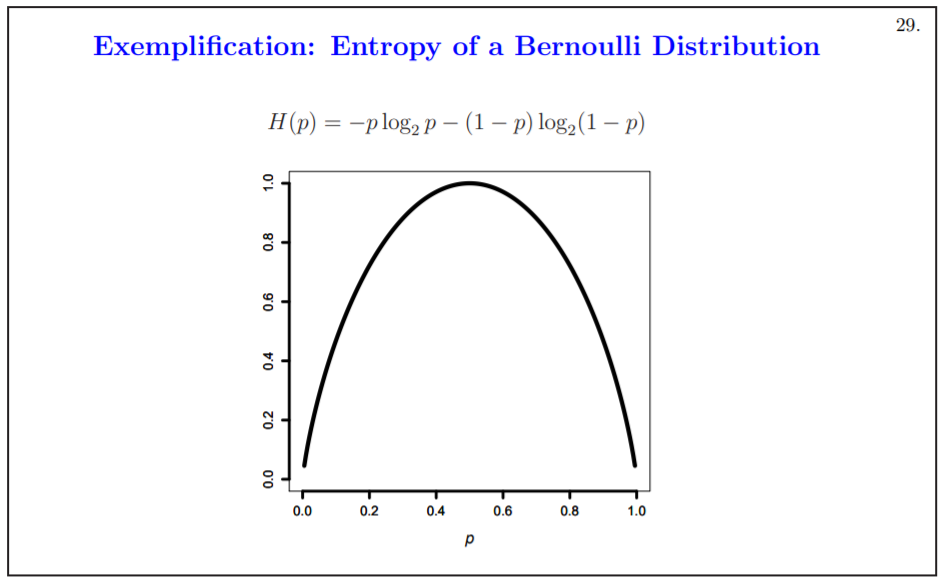
\includegraphics[width=1\linewidth]{screenshot001}
					(slide preluat din \url{https://profs.info.uaic.ro/~ciortuz/SLIDES/foundations.pdf})
				\end{center}
				vom putea:
				\begin{itemize}
					\item spune că $H[5-,3+] = H[5+,3-]$
					\item compara $H[5-,3+]$ cu $H[2-,9+]$ fără a face calcule prea multe: vom compara $\frac{\min(5,3)}{5+3} = \frac{3}{8} = \frac{33}{88}$ cu $\frac{\min(2,9)}{2+9} = \frac{2}{11} = \frac{16}{88}$; cum $\frac{33}{88} > \frac{16}{88}$, vom avea: $H[5-,3+] > H[2-,9+]$
					\item la fel, putem compara $H[4-,5+]$ cu $H[5-,6+]$: $\frac{\min(4,5)}{4+5}$ cu $\frac{\min(5,6)}{5+6}$, adică $\frac{4}{9}$ cu $\frac{5}{11}$, adică $\frac{44}{99}$ cu $\frac{45}{99}$. Cum $\frac{44}{99} < \frac{45}{99}$, avem: $H[4-,5+] < H[5-,6+]$
				\end{itemize}
				\item \begin{center}
					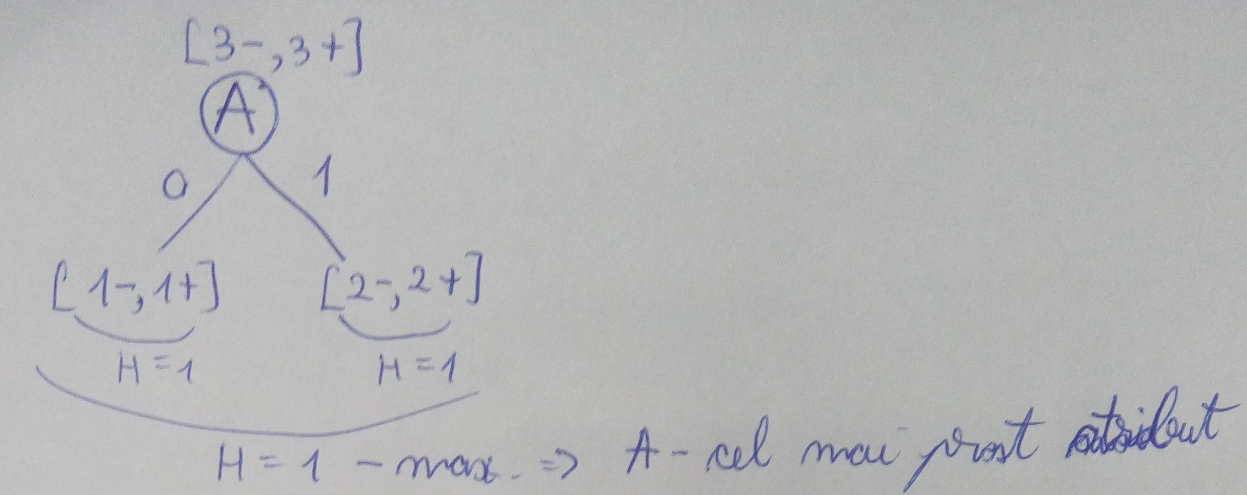
\includegraphics[width=1\linewidth]{screenshot003}
				\end{center}
				\item \begin{center}
					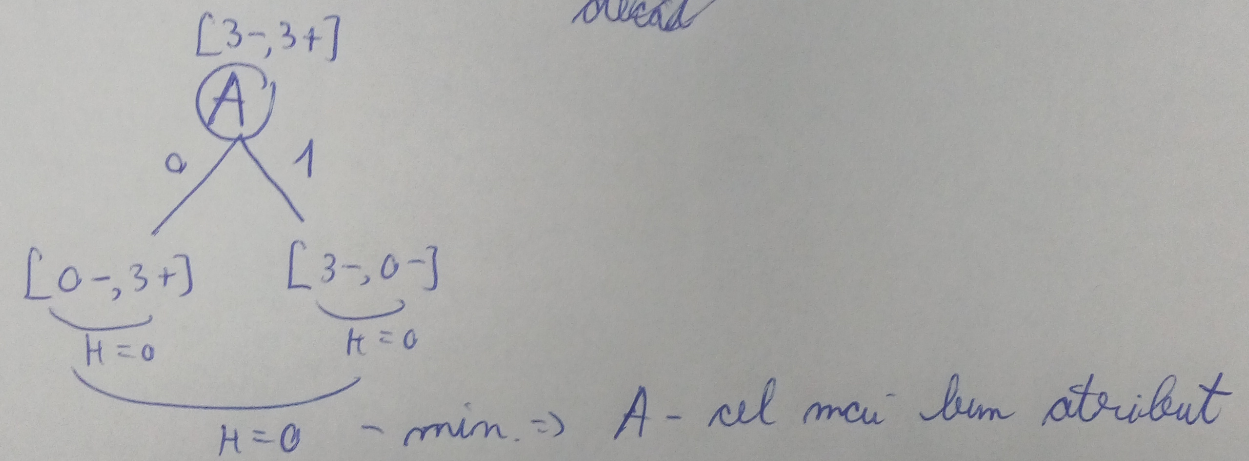
\includegraphics[width=1\linewidth]{screenshot004}
				\end{center}
				\item La pagina 269 din culegere aveți undeva:
				\begin{center}
					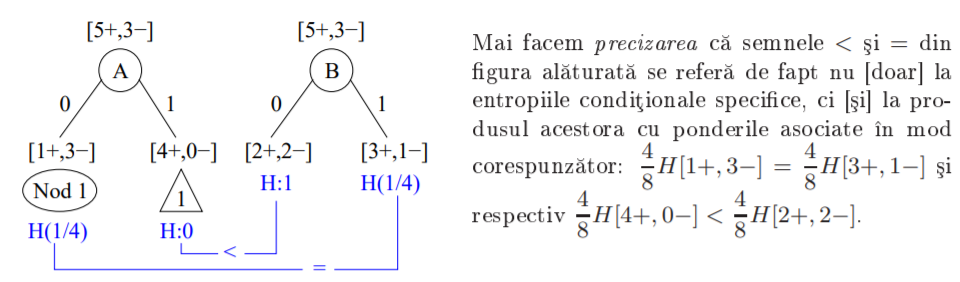
\includegraphics[width=1\linewidth]{screenshot002}
				\end{center}
				Veți putea compara compași de decizie fără calcule în anumite situații, dar nu uitați că semnele de $>$, $<$, $=$ se referă \textbf{nu doar la entropii, cât și la ponderi}. Vedeți și următoarele exemple:
				\begin{center}
					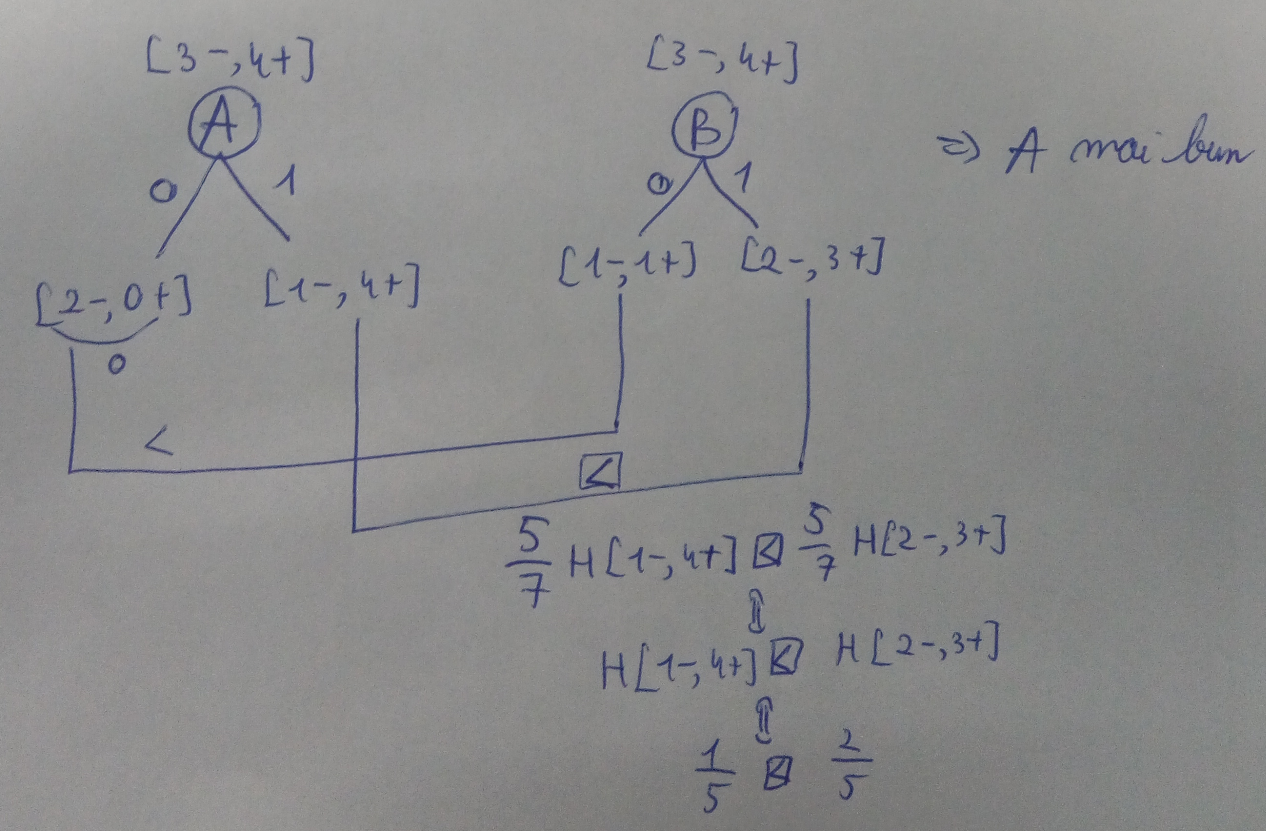
\includegraphics[width=1\linewidth]{screenshot005}
				\end{center}
				\begin{center}
					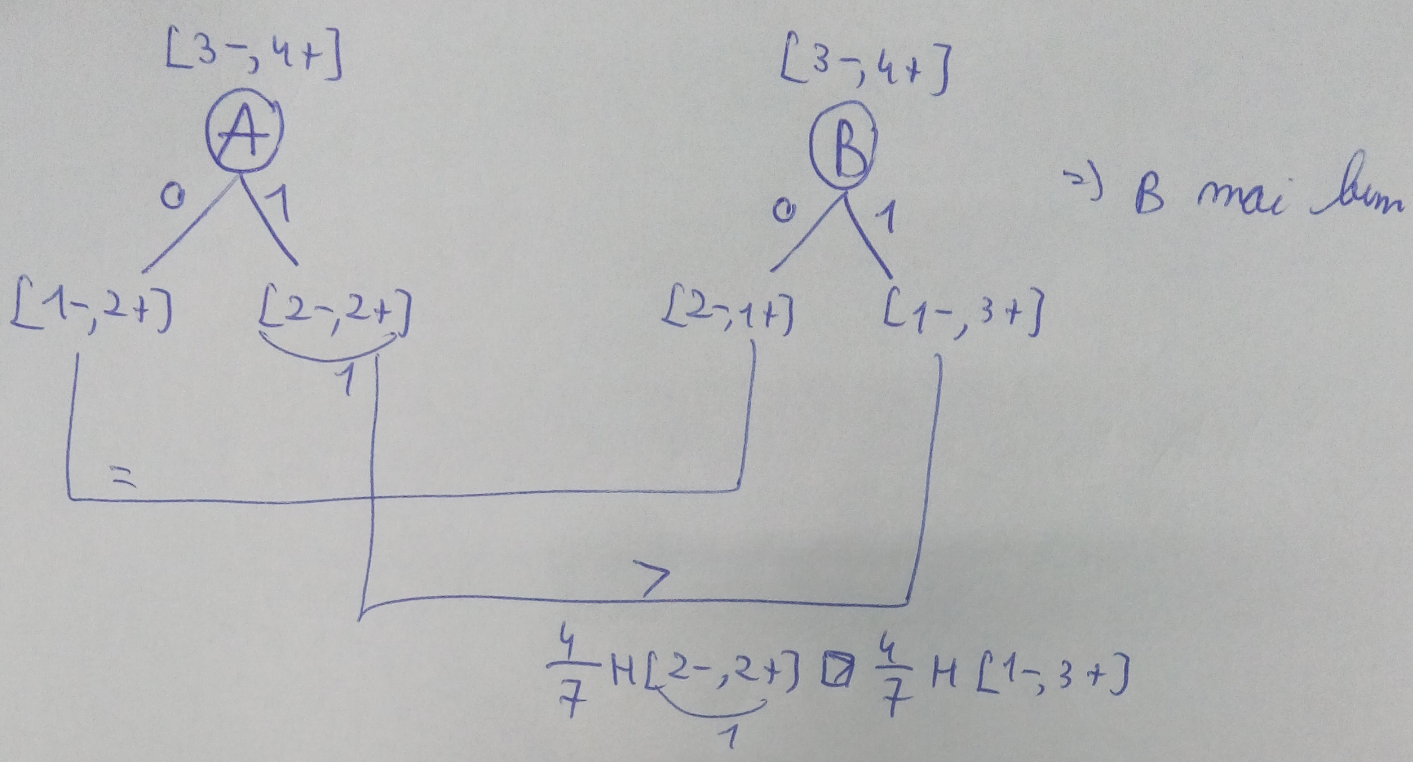
\includegraphics[width=1\linewidth]{screenshot006}
				\end{center}
				\begin{center}
					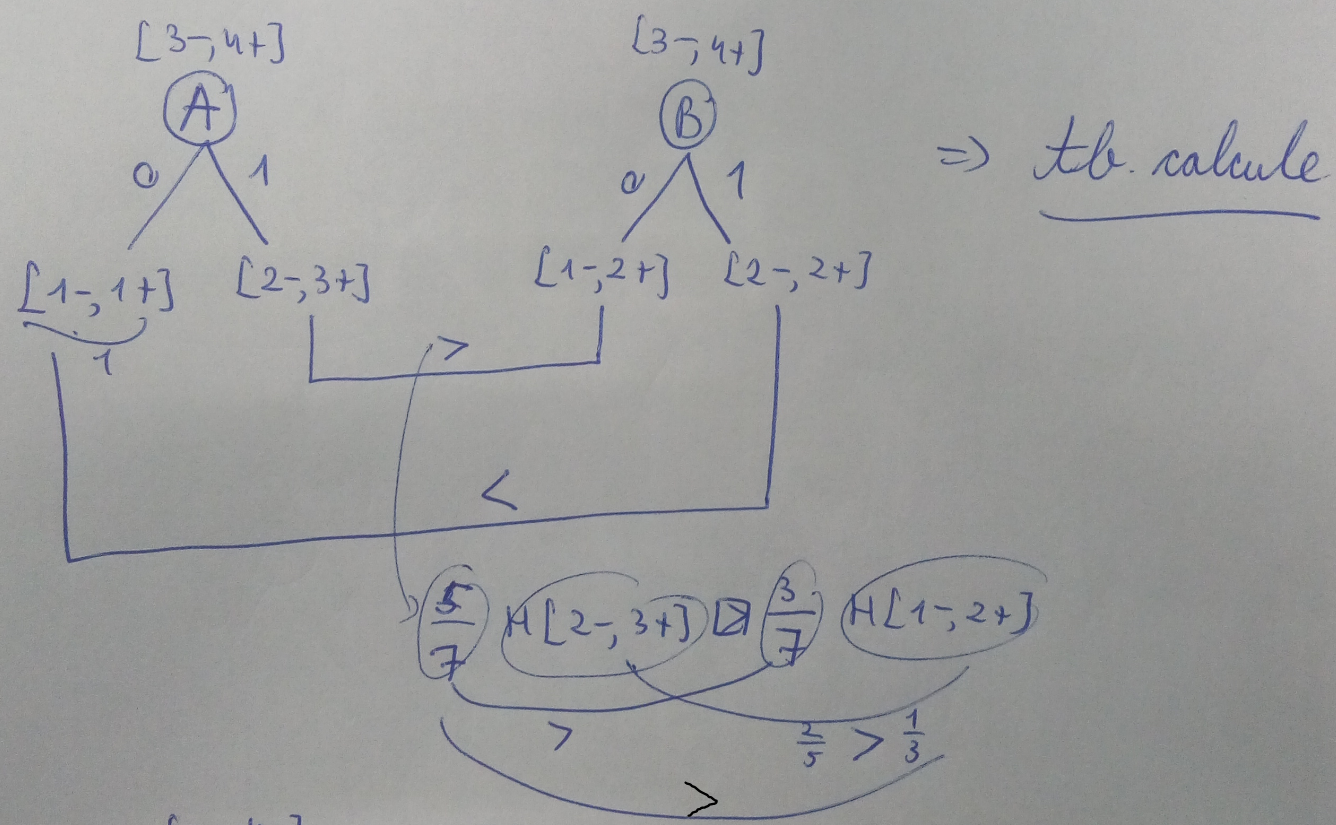
\includegraphics[width=1\linewidth]{screenshot007}
				\end{center}
				\begin{center}
					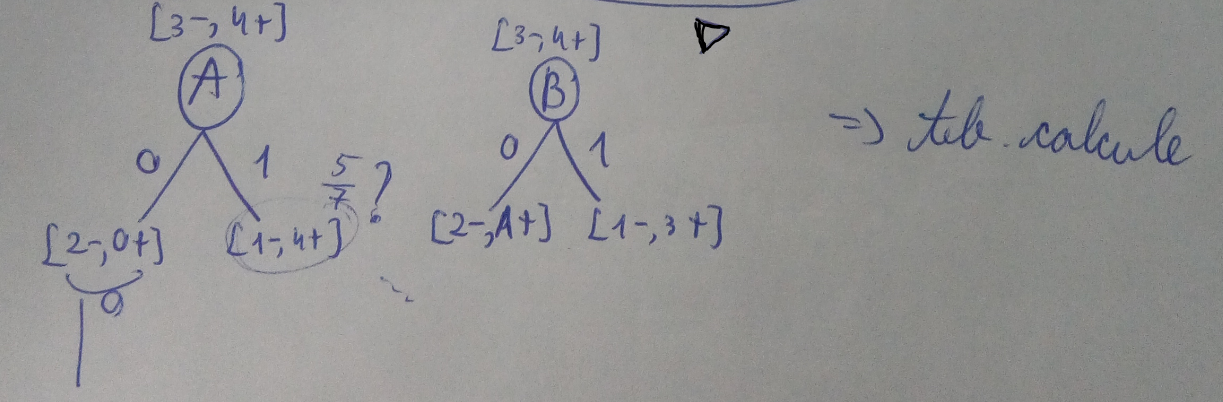
\includegraphics[width=1\linewidth]{screenshot008}
				\end{center}
				
			\end{itemize}
		\end{enumerate}
	\end{enumerate}
	
	\textbf{Observație}: rezolvări de tipul \textit{mi se pare că nodul acesta va da IG-ul cel mai mare (pentru că are un nod frunză deja etc.)} nu se punctează. Ori faceți calcule, ori faceți un raționament calitativ valid (ca mai sus sau altele nemenționate aici: simetria pentru o formula booleană etc.).
	
	\textbf{\large{Extensie ID3 - lucru cu atribute continue}}
	
	vezi ex.10/pag.279
	
	vezi ex.12/pag.282
	
	
	\newpage
	\textbf{\large{Schemă de final}}
	\begin{enumerate}
		\item Învățare supervizată de tip clasificare (2)
		\begin{enumerate}
			\item antrenare
			\item testare
			\item validare
			\item cross-validare cu metoda k-fold
			\item cross-validare cu metoda leave-one-out
		\end{enumerate}
		\item ID3 (2)
			\begin{enumerate}
				\item eroarea la antrenare pe set de date consistent/inconsistent
				\item eroarea la CVLOO
			\end{enumerate}
		\item ID3 (2) - calcule mai rapide
			\begin{enumerate}
				\item formule ex.33/pag.331 - vezi filmulețe fb
				\item raționamente calitative
			\end{enumerate}
		\item Extensie ID3 - lucru cu atribute continue
	\end{enumerate}
	
\end{document}